\documentclass[A4, 12pt]{article}

\usepackage{stdcd}

% title info
\title{Digital Communications -- Assignment 1}
\author{Cian Dowd}
\date{\today}

\begin{document}
\maketitle

\section{Deriving Theoretical Error Rates}
To find the probability of error in a single dimension we use

\begin{equation*}
	p_e = Q \left( \frac{d}{2 \sigma} \right)
\end{equation*}

Where the Q function is 
\begin{equation*}
	Q(x) = \int_{x}^{\infty} \frac{1}{\sqrt{2\pi}} \exp \left(\frac{-z^2}{2} \right) dx
\end{equation*}

The probability of error in two dimensions depends on the decision boundaries around a symbol.
We can see that there are two sets, of four symbols each, for which there are matching symbols.
The probability of error for these sets is given in Equations \ref{eq:corner} and \ref{eq:middle}

\begin{equation}
	p(Error \mid s_i) = 2 \cdot Q \left( \sqrt{ \frac{E_s}{3 N_o} } \right) - Q^2 \left( \sqrt{ \frac{E_s}{3 N_o} } \right) , i = \{1,2,7,8\}
	\label{eq:corner}
\end{equation}

\begin{equation}
	p(Error \mid s_i) = 3 \cdot Q \left( \sqrt{ \frac{E_s}{3 N_o} } \right) - 2 \cdot Q^2 \left( \sqrt{ \frac{E_s}{3 N_o} } \right) , i = \{3,4,5,6\}
	\label{eq:middle}
\end{equation}

\subsection{\ac{ser}}
For \ac{ser} we can see that the average \ac{ser} is the weighted average of Equations \ref{eq:corner} and \ref{eq:middle}.
Following this we can see that the theoretical \ac{ser} is given by Equation \ref{eq:serfin}.

\begin{equation*}
	\begin{split}
		p_e = \frac{1}{8}
		\Bigg[
			4 \left[ 2 \cdot Q \left( \sqrt{ \frac{E_s}{3 N_o} } \right) - Q^2 \left( \sqrt{ \frac{E_s}{3 N_o} } \right) \right]\\
			+ 4 \left[ 3 \cdot Q \left( \sqrt{ \frac{E_s}{3 N_o} } \right) - 2 \cdot Q^2 \left( \sqrt{ \frac{E_s}{3 N_o} } \right) \right]
		\Bigg]
	\end{split}
\end{equation*}

\begin{equation}
	\begin{split}
		p_e = \frac{1}{2}
		\Bigg[
			5 \cdot Q \left( \sqrt{ \frac{E_s}{3 N_o} } \right) - 3 \cdot Q^2 \left( \sqrt{ \frac{E_s}{3 N_o} } \right)
		\Bigg]
	\end{split}
	\label{eq:ser}
\end{equation}

\begin{equation}
	\begin{split}
		p_e =
		\Bigg[
			\frac{5}{2} \cdot Q \left( \sqrt{ \frac{E_s}{3 N_o} } \right) - \frac{3}{2} \cdot Q^2 \left( \sqrt{ \frac{E_s}{3 N_o} } \right)
		\Bigg]
	\end{split}
	\label{eq:serfin}
\end{equation}

\subsection{\ac{ber}}
As $E_b = \frac{E_s}{3}$ then $Q \left( \sqrt{ \frac{E_s}{3 N_o} } \right)$ becomes $Q \left( \sqrt{ \frac{E_b}{3 N_o} } \right)$.
Where we previously averaged across 8 signals we now have 24 bits, 3 bits per symbol.
Noting these differences, Equation \ref{eq:ber} is the \ac{ber} equivalent of Equation \ref{eq:ser} and the theoretical \ac{ber} is given by Equation \ref{eq:berfin}.

\begin{equation}
	\begin{split}
		p_e = \frac{1}{2 \cdot 3}
		\Bigg[
			5 \cdot Q \left( \sqrt{ \frac{E_b}{N_o} } \right) - 3 \cdot Q^2 \left( \sqrt{ \frac{E_b}{N_o} } \right)
		\Bigg]
	\end{split}
	\label{eq:ber}
\end{equation}

\begin{equation}
	\begin{split}
		p_e =
		\frac{5}{6} \cdot Q \left( \sqrt{ \frac{E_b}{N_o} } \right) - \frac{1}{2} \cdot Q^2 \left( \sqrt{ \frac{E_b}{N_o} } \right)
	\end{split}
	\label{eq:berfin}
\end{equation}

\section{Transmitter Encoding Scheme}

The mapping of bits to symbols was done with a Gray Code, seen in Table \ref{tab:gray}.
This serves several purposes:

\begin{itemize}
	\item If a symbol is in error with a neighbouring symbol there is only one bit error
	\item It is possible to map each bit in the three bit word to a direction decision
\end{itemize}

\begin{table}[H]
	\centering
	\caption{Gray-Coding Scheme}
	\begin{tabular}{ c c }
		000 & 100\\
		001 & 101\\
		011 & 111\\
		010 & 110\\
	\end{tabular}
	\label{tab:gray}
\end{table}

It is clear from Table \ref{tab:gray} that any neighbouring errors only result in a bit error.
\par
Table \ref{tab:bit} and Figure \ref{fig:treesig} show how the code maps words to symbols.
It is used to generate the correct signal and for the transmitter to know what was sent.
This can be seen also by comparing the descriptions in Table \ref{tab:bit} with the positions of the words in Table \ref{tab:gray}.

\begin{table}[H]
	\centering
	\caption{The Roll of Each Bit in Symbol Mapping}
	\begin{tabular}{r  l  l}
		& \textbf{Bit is 0} & \textbf{Bit is 1}\\
		\textbf{1\textsuperscript{st} Bit} & Negative half plane of $x$ axis & Positive half plane of $x$ axis \\
		\textbf{2\textsuperscript{nd} Bit} & Positive half plane of $y$ axis & Negative half plane of $y$ axis \\
		\textbf{3\textsuperscript{rd} Bit} & Most extreme $y$ position & Least extreme $y$ position \\
	\end{tabular}
	\label{tab:bit}
\end{table}

\begin{figure}[H]
	\centering
	\begin{minipage}{.4\textwidth}
		\centering
        \captionsetup{width=1\linewidth,justification=centering}
		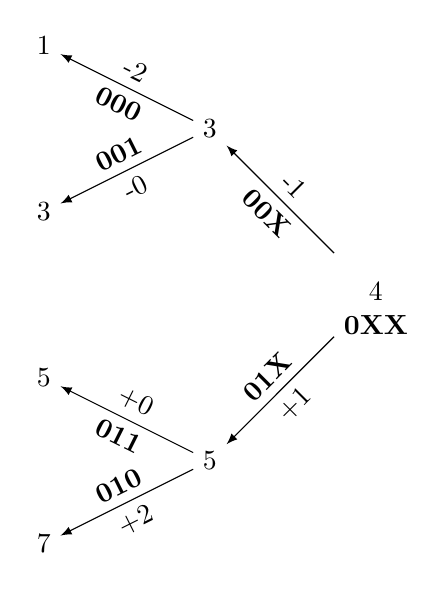
\begin{tikzpicture}
			[
				grow                    = left,
				level distance          = 6em,
				edge from parent/.style = {draw, -latex},
				align					= center,
				sloped
			]
			\tikzstyle{level 1}=[sibling distance=12em]
			\tikzstyle{level 2}=[sibling distance=6em]
			\node [] {\\[1ex]4\\\textbf{0XX}}
				child { node [] {3}
					child { node [] {1}
						edge from parent node [above] {-2}
										 node [below] {\textbf{000}} }
					child { node [] {3}
						edge from parent node [below] {-0}
										 node [above] {\textbf{001}} }
					edge from parent node [above] {-1} 
									 node [below] {\textbf{00X}} }
				child { node [] {5}
					child { node [] {5}
						edge from parent node [above] {+0}
										 node [below] {\textbf{011}} }
					child { node [] {7}
						edge from parent node [below] {+2} 
										 node [above] {\textbf{010}} }
					edge from parent node [below] {+1}
									 node [above] {\textbf{01X}} };
		\end{tikzpicture}
		\caption*{Decision Tree if First Bit is 0}
	\end{minipage}
	\begin{minipage}{.4\textwidth}
		\centering
        \captionsetup{width=1\linewidth,justification=centering}
		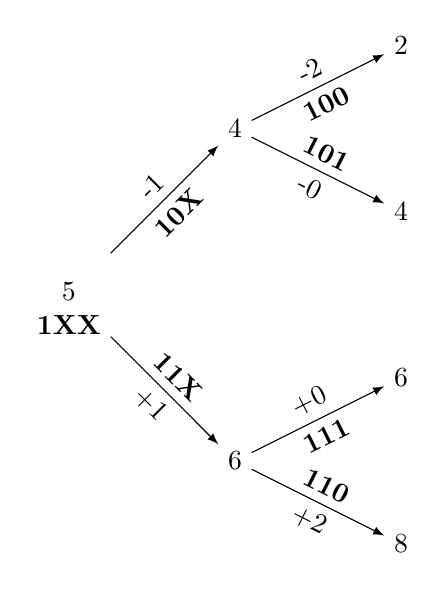
\begin{tikzpicture}
			[
				grow                    = right,
				level distance          = 6em,
				edge from parent/.style = {draw, -latex},
				align					= center,
				sloped
			]
			\tikzstyle{level 1}=[sibling distance=12em]
			\tikzstyle{level 2}=[sibling distance=6em]
			\node [] {\\[1ex]5\\\textbf{1XX}}
				child { node [] {6}
					child { node [] {8}
						edge from parent node [below] {+2} 
										 node [above] {\textbf{110}} }
					child { node [] {6}
						edge from parent node [above] {+0}
										 node [below] {\textbf{111}} }
					edge from parent node [below] {+1}
									 node [above] {\textbf{11X}} }
				child { node [] {4}
					child { node [] {4}
						edge from parent node [below] {-0}
										 node [above] {\textbf{101}} }
					child { node [] {2}
						edge from parent node [above] {-2}
										 node [below] {\textbf{100}} }
					edge from parent node [above] {-1} 
									 node [below] {\textbf{10X}} };
		\end{tikzpicture}
		\caption*{Decision Tree if First Bit is 1}
	\end{minipage}
	\caption{Decision Tree for Tracking Signal Enumeration During Modulation}
	\label{fig:treesig}
\end{figure}

Figure \ref{fig:treesym} shows how the bits in the words, following the descriptions in Table \ref{tab:bit}, generates the signal piecewise, reading one bit at a time.

\begin{figure}[H]
	\centering
	\begin{tikzpicture}
		[
			grow cyclic,
			rotate					= -90,
			level distance          = 7em,
			edge from parent/.style = {draw, -latex},
			align					= center,
			sloped
		]
		\tikzstyle{level 1}=[sibling angle=180]
		\tikzstyle{level 2}=[sibling angle=180]
		\tikzstyle{level 3}=[level distance=14em]
		\node [] {$(0,0)$}
					child { node [] {$(-\frac{d}{2},0)$}
						child { node [] {$s_3 = (-\frac{d}{2},\frac{d}{2})$}
							child { node [] {$s_1 = (-\frac{d}{2},\frac{3 d}{2})$}
								edge from parent node [left] {$+(0,\frac{2 d}{2})$}
												 node [right] {\textbf{000}} }
							edge from parent node [left] {$+(0,\frac{d}{2})$}
											 node [right] {\textbf{00X}} }
						child { node [] {$s_5 = (-\frac{d}{2},-\frac{d}{2})$}
							child { node [] {$s_7 = (-\frac{d}{2},-\frac{3 d}{2})$}
								edge from parent node [left] {$+(0,-\frac{2 d}{2})$}
												 node [right] {\textbf{010}} }
							edge from parent node [left] {$+(0,-\frac{d}{2})$}
											 node [right] {\textbf{01X}} }
						edge from parent node [below] {$+(-\frac{d}{2},0)$}
										 node [above] {\textbf{0XX}} }
					child { node [] {$(\frac{d}{2},0)$}
						child { node [] {$s_6 = (\frac{d}{2},-\frac{d}{2})$}
							child { node [] {$s_8 = (\frac{d}{2},-\frac{3 d}{2})$}
								edge from parent node [right] {$+(0,-\frac{2 d}{2})$}
												 node [left] {\textbf{110}} }
							edge from parent node [right] {$+(0,-\frac{d}{2})$}
											 node [left] {\textbf{11X}} }
						child { node [] {$s_4 = (\frac{d}{2},\frac{d}{2})$}
							child { node [] {$s_2 = (\frac{d}{2},\frac{3 d}{2})$}
								edge from parent node [right] {$+(0,\frac{2 d}{2})$}
												 node [left] {\textbf{100}} }
							edge from parent node [right] {$+(0,\frac{d}{2})$}
											 node [left] {\textbf{10X}} }
						edge from parent node [below] {$+(-\frac{d}{2},0)$}
										 node [above] {\textbf{1XX}} };
	\end{tikzpicture}
	\caption{Decision Tree for Modulating 3-Bit Words to Signals}
	\label{fig:treesym}
\end{figure}

The MATLAB script uses the decision trees shown in both Figure \ref{fig:treesig} and Figure \ref{fig:treesym} to generate the signal to transmit and to know what that signal is, for checking error rate once it is received.

\section{Results}

\subsection{\ac{ser} Below $10^{-4}$}
The \ac{ser} lies below $10^{-4}$ for $E_s/N_o$ of $\sim$\SI{16.7}{\decibel}.

\subsection{\ac{ber} Below $10^{-4}$}
The \ac{ber} lies below $10^{-4}$ for $E_b/N_o$ of $\sim$\SI{11.2}{\decibel}.

\subsection{Graphs}
Figures \ref{fig:ser} and \ref{fig:ber} graph the \ac{ser} and \ac{ber} respectively while Figures \ref{fig:sererror} and \ref{fig:bererror} show the percentage error between the theoretical and actual values.
With both \ac{ser} and \ac{ber} show the percentage error increases towards the end while \ac{ber} has more errors at the start. 
There are greater actual errors with the \ac{ber} than the theoretical errors as the model only accounts for single-bit errors.
These errors are more common at high SNR which is why the actual errors are greater for low SNR, where a symbol can be in error but cause more than a single-bit error.

\begin{figure}[H]
	\centering
	\begin{minipage}{.4\textwidth}
		\centering
		\includegraphics[width=7cm]{../images/ser}
		\caption{\ac{ser}}
		\label{fig:ser}
	\end{minipage}
	\begin{minipage}{.4\textwidth}
		\centering
		\includegraphics[width=7cm]{../images/sererror}
		\caption{\ac{ser} Error}
		\label{fig:sererror}
	\end{minipage}
\end{figure}

\begin{figure}[H]
	\centering
	\begin{minipage}{.4\textwidth}
		\centering
		\includegraphics[width=7cm]{../images/ber}
		\caption{\ac{ber}}
		\label{fig:ber}
	\end{minipage}
	\begin{minipage}{.4\textwidth}
		\centering
		\includegraphics[width=7cm]{../images/bererror}
		\caption{\ac{ber} Error}
		\label{fig:bererror}
	\end{minipage}
\end{figure}

\end{document}
